%
% 講演資料
%  https://scrapbox.io/masui/ソフトウェア科学会_基礎研究賞講演_2021/9/3
% Cloud LaTeX
%  https://cloudlatex.io/projects/411855/edit
% 記事依頼
%  https://mail.google.com/mail/u/0/?zx=a0kk8p4fqhm3#inbox/WhctKKWxdNgXpJNJdpfrtHgVMQJTthSKpCLwgCTppBnkqJbWZmmsxwzHgMwmjcxmLrKmfZV
% 執筆要項 (スタイルファイル)
%  https://www.jssst.or.jp/edit/detail/style_files.html
% 記事例
%  https://s3-ap-northeast-1.amazonaws.com/masui.org/f/5/f5361cf93c65dd661e5797ed105bfeca.pdf
%

\long\def\comment#1{}

\documentclass[topics]{compsoft} % トピックス

% 「コンピュータソフトウェア」誌に掲載される論文の場合,次で巻数,号数,開始ページ,終了ページを指定する.
\volNoPp{30}{1}{78}{84}

% \usepackage[dvips]{graphics}

\usepackage{graphicx}

\usepackage{here} % [H]とするとその場所に配置されるらしい

\begin{document}

\title{ユニバーサルなユーザインタフェース}

% 著者
% 和文論文の場合,姓と名の間には半角スペースを入れ,
% 複数の著者の間は全角スペースで区切る
%
\author{増井 俊之
%
% ここにタイトル英訳 (英文の場合は和訳) を書く.
%
\ejtitle{Concurrent Operations on Splay Trees.}
%
% ここに著者英文表記 (英文の場合は和文表記) および
% 所属 (和文および英文) を書く.
% 複数著者の所属はまとめてよい.
%
\shozoku{Kazunori Ueda}{慶應義塾大学 環境情報学部}%
{Dept.\ of Information and Computer Science, Waseda University}
%
% 出典情報は \shutten とすれば出力される.
\shutten
%
% 受付年月日,記事カテゴリなどは自動的に生成される.
\uketsuke{2021}{11}{15}
%
% その他,脚注に入れるものがあれば,\note に記述する.
%\note{脚注に入れる内容}
}

% 和文アブストラクト
\Jabstract{%
ユーザインタフェースとは
}
%
% 英文アブストラクト(本サンプルの原論文にはなし)
\Eabstract{%
We talk ablut uniersal UI.
%
}

\maketitle

\section{はじめに}

私は30年以上にわたり、コンピュータの使い勝手を改善する
ユーザインタフェースの研究開発を行なってきました。
このことが評価され、2020年度日本ソフトウェア科学会基礎研究賞を頂くことができ、
大変光栄に思っております。
受賞業績のタイトルである「ユニバーサルなユーザインタフェース」について、
世の中の動向および私自身の研究について紹介させていただきます。

昔のコンピュータは専門家が使うものでしたが、
最近は誰もががパソコンやスマホでコンピュータやインターネットを活用しています。
これはコンピュータのユーザインタフェースの改良の結果です。
コンピュータが世の中で使われはじめた頃は
文字ベースの入出力(Command Line Interface: CLI)が一般的でしたが、
1970年代に高解像度ディスプレイの上の
「ウィンドウ」や「メニュー」などを利用する
「グラフィカルユーザインタフェース」(Graphical User Interface: GUI)がXerox PARCで発明されて以来
コンピュータ利用のハードルが低くなり、
現在は多くの人々がコンピュータを使えるようになってきたといえるでしょう。

近年のコンピュータ利用のトレンドを表現するキーワードとして
「モバイルコンピューティング」や「ユビキタスコンピューティング」といったものがあります。
これらはコンピュータを誰でもいつでも使うというニュアンスがあり、
コンピュータが「ユニバーサル」に使えるようになってきたことのあらわれでしょう。
%
「ユニバーサル」というのは、
障害や年齢などにかかわらず「誰でも使える」という意味です。
例えば、障害があっても言葉が通じなくても「自動ドア」を使うことができますから、
自動ドアはユニバーサルに利用できるインタフェースだと言うことができます。
%
誰でも使えるユニバーサルなシステムを設計することは
「ユニバーサルデザイン」と呼ばれ、
近年この考え方の重要性が広く認識されるようになりました。

\comment{
ユニバーサルデザインの考え方はコンピュータに限ったものではありません。
最近建築される家屋は段差が無いように設計されているものが多く、
歩行が得意でない人間でも生活しやすいようになっていますが、
これは建築におけるユニバーサルデザインです。
%
家の中の段差などは誰にとっても邪魔なものであり、
こういう問題を解決するための
ユニバーサルデザインはあらゆる人にとって有益なはずです。
}

% 特定の障害を念頭に置かず、
% 常にあらゆる人が利用できるシステムを設計することが重要だということが認識されてきたように思われます。

\comment{
これまでのコンピュータは
高度な計算、大量の記憶、コミュニケーションのサポート、情報入力/編集のサポート、
情報検索のサポートなど様々な用途に利用されてきましたが、
おおざっぱに言うと、
コンピュータは「人間の弱点を補強する」ために広く利用されてきたということができるかもしれません。

以前は専門家の仕事を補助するために、
また現在は一般人が苦手としていることを助けるために、
人々の弱点を補強する用途として利用されているわけです。
将来は、さらに広い領域で人々をサポートするために
コンピュータが使われることがもっと増えてくることでしょう。
}

近年、「Augmented Human」というキーワードで
研究が行なわれたりコンファレンスが開かれたりしています\footnote{
  \textsf{https:{\slash}{\slash}www.augmented-human.com{\slash}}
}。
これは「人間の能力をコンピュータで拡張する」というコンセプトです。
これは新しい言葉ですが、
様々な技術で
人を助けたり能力を増強したりするという考えは新しいものではありません。
服もメガネも自動車も文房具も、すべてその範疇であり、
大きな産業になっています。

私がユーザインタフェースの研究をはじめた1980年代は
まだまだ計算機は専門家が使うものだと思われており、
誰もが使えるものを作るといった考えはあまりポピュラーではありませんでした。
%
しかし将来は
あらゆる人間の弱点を補強したり能力を拡張したりするという用途に
広くコンピュータが利用されてくることは間違いありません。
ユニバーサルデザインにもとづいて
人間を補助するために
コンピュータが今後より多く利用されていくことは間違いないでしょう。

 
\section{ユニバーサルなシステム開発例}

私は「ユニバーサル」であることを重視した
インタフェースシステムを開発したり普及を試みたりしてきています。
そのようなシステムの実例をいくつか紹介させていただきます。

\subsection{テキスト入力支援}

私は2000年ごろ、
普及しつつあった携帯電話のための
予測型日本語入力手法「POBox」\footnote{
  \textsf{https:{\slash}{\slash}ja.wikipedia.org{\slash}wiki{\slash}POBox}
}を製品化しました。

\begin{figure}[h]
  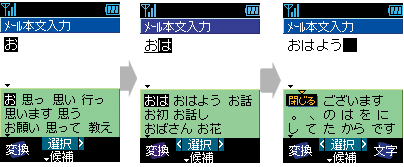
\includegraphics[width=10cm,bb=0 0 404 600]{figures/ac2b347a7042f920edd576ee07c4b7f4.png}
  \caption{POBox.}
  \label{example1}
\end{figure}

コンピュータが人間の操作を予測することにより
人間の負担を減らす「予測インタフェース」システムの研究が
従来から行なわれていましたが\cite{WatchWhatIDo}\cite{YourWish}、
POBoxはこれをテキスト入力に応用したものです。
%
予測型入力システムは、携帯電話のような小型のモバイル機器での
テキスト入力に便利だということが評価され、
現在の携帯機器でのテキスト入力手法の標準となっています。

テキスト入力に予測インタフェースを利用するという手法は、
障害者向けの入力インタフェースとして従来から利用されていましたが、
POBoxは、誰もが使えるユニバーサルなインタフェースとしてデザインされているところが重要です。
ユニバーサルなユーザインタフェースの工夫によって
あらゆる人々が使えるシステムを作ることが可能になることを示せた点は意義があったと考えています。

現在、予測型テキスト入力手法は
各種スマホの入力手法や
障害者用入力システムPETE\footnote{
  \textsf{https:{\slash}{\slash}www.ideafront.jp{\slash}PeteHP{\slash}}
}
などでも利用されています。

\begin{figure}[h]
  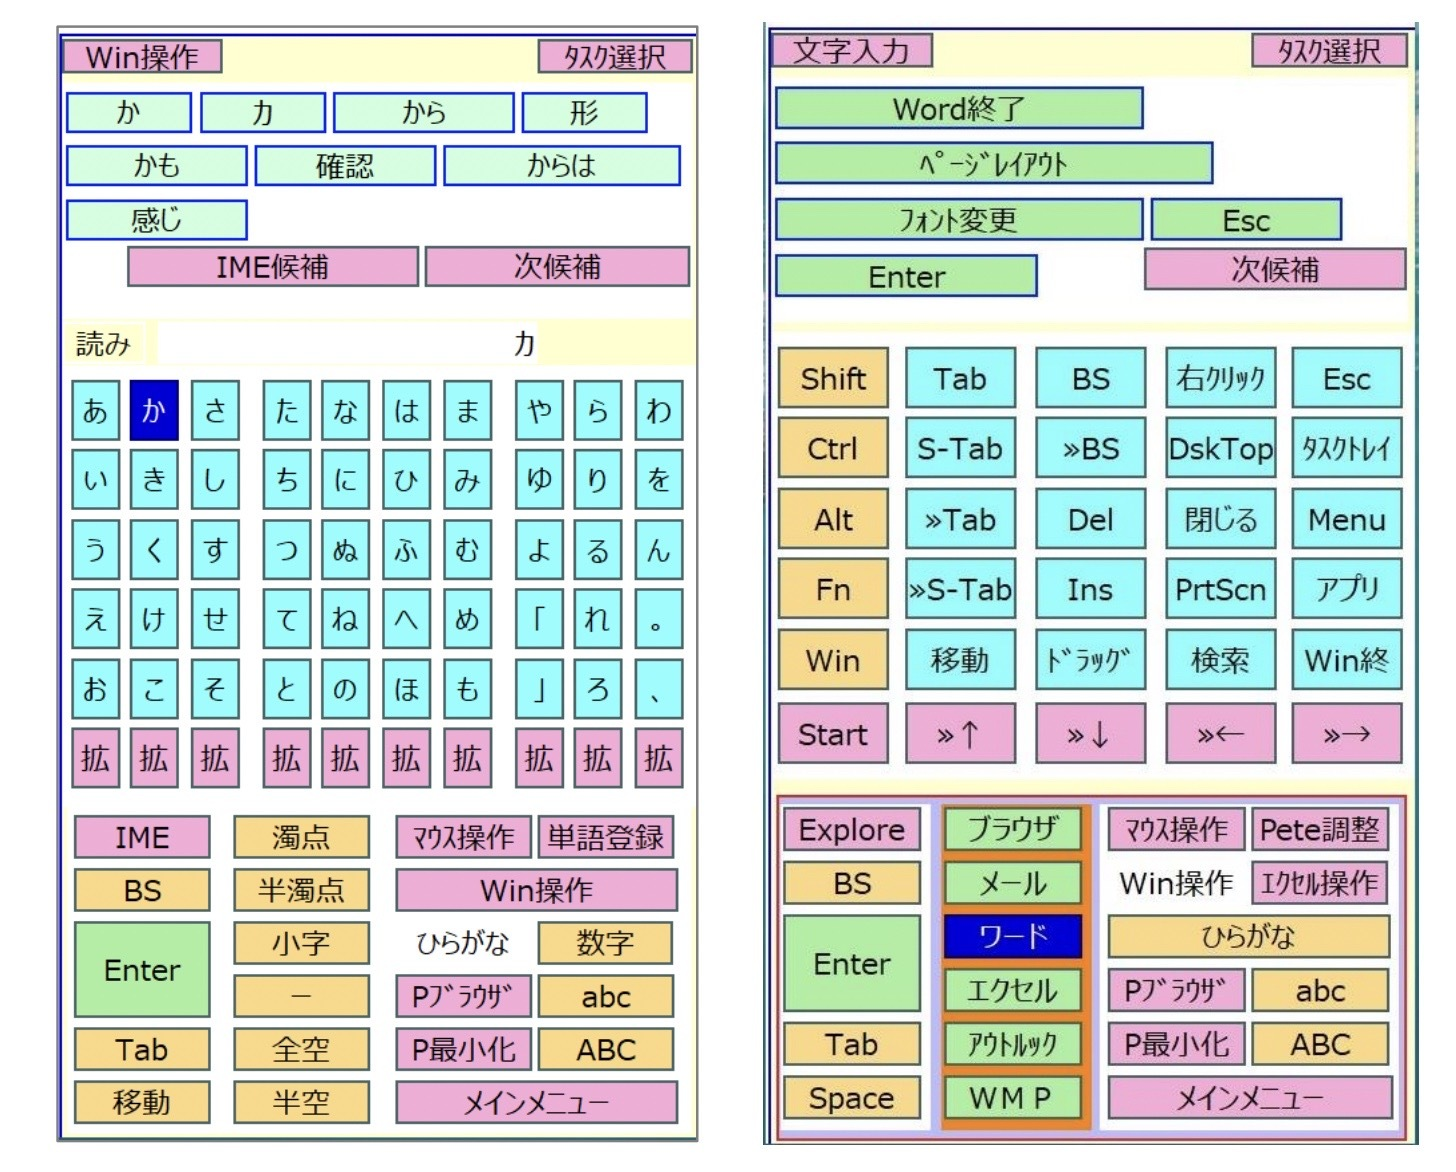
\includegraphics[width=9cm,bb=0 0 1456 1172]{figures/a2f652e2f488b96974e92f8198f49469.jpg}
  \caption{PETE利用画面.}
  \label{pete}
\end{figure}

\subsection{画面キャプチャ}

パソコンの画面の一部を保存したり共有したりしたいことがよくあります。
大抵のパソコンには画面をキャプチャする機能がありますが、
キャプチャした画像をWebなどで使ったり他人と共有したりすることは
意外と面倒でした。
画面上で領域を選択すると、
すぐその画像がWeb上にアップロードされて固有のURLが付加される
「Gyazo」というソフトウェア\footnote{
  \textsf{https:{\slash}{\slash}Gyazo.com{\slash}}
}を2007年に開発して公開しました。

Gyazoを使うととても単純な操作で画像を活用することができるので
ユーザ数が爆発的に増加を続け、
現在は全世界で月間1000万人のユーザに利用されています。

Gyazoでは画像キャプチャ時にアプリケーション情報などの付帯情報や
OCRテキストを記録するため、
画像をキャプチャするだけで様々な情報整理を行なうこともできます。

Webのトラフィック情報を計測するAlexa\footnote{
  \textsf{https:{\slash}{\slash}www.alexa.com{\slash}}
}のデータによると、
Gyazoは全Webサービスで数百番目にトラフィックが多いサービスになっています。

\begin{figure}[h]
  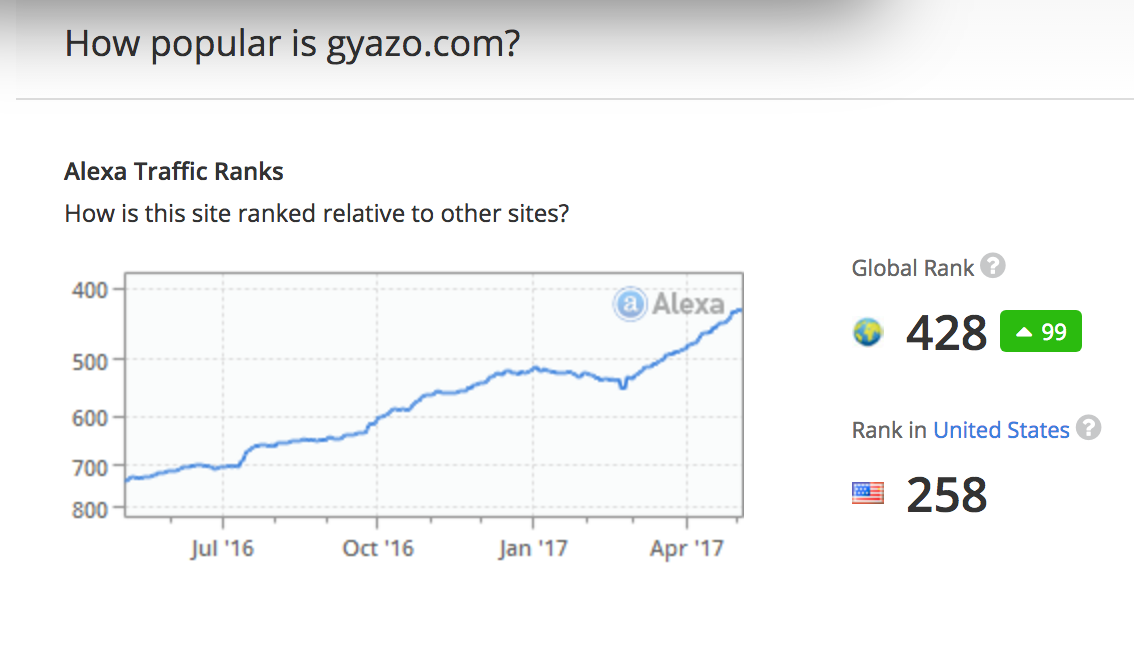
\includegraphics[width=9cm,bb=0 0 1134 668]{figures/2595e48e8346b423d6e6c1d23daf10f4.png}
  \caption{Gyazoのトラフィック遷移.}
  \label{alexa}
\end{figure}


\subsection{思考支援}

アイデアをまとめたり文章を書いたりするのは大変な作業です。
ワープロ、{\TeX}、HTMLなどを使ってコンピュータで綺麗な文章を作ることはできますし、
アイデアや考えをまとめるためのシステムやサービスが近年多数提案されていますが、
決定版といえるものはまだ無く、試行錯誤している人も多いと思います。

頭の中の考えをまとめたいときや
情報を共有したいとき、
「Wiki」を使うと効果的だと考え、
Gyazz\cite{Gyazz}というシステムを作成して長年利用してきました。
現在は「Scrapbox」\footnote{scrapbox}という名前で商品化しています。
Scrapboxは、
ブラウザ上でリアルタイムに手軽に情報を共有することができるサービスです。
複数ユーザが同時にテキスト編集を行なえることに加え、
ページ間のリンクを簡単に作ることができるので、
様々な用途に使うことができます。

\begin{figure}[t]
  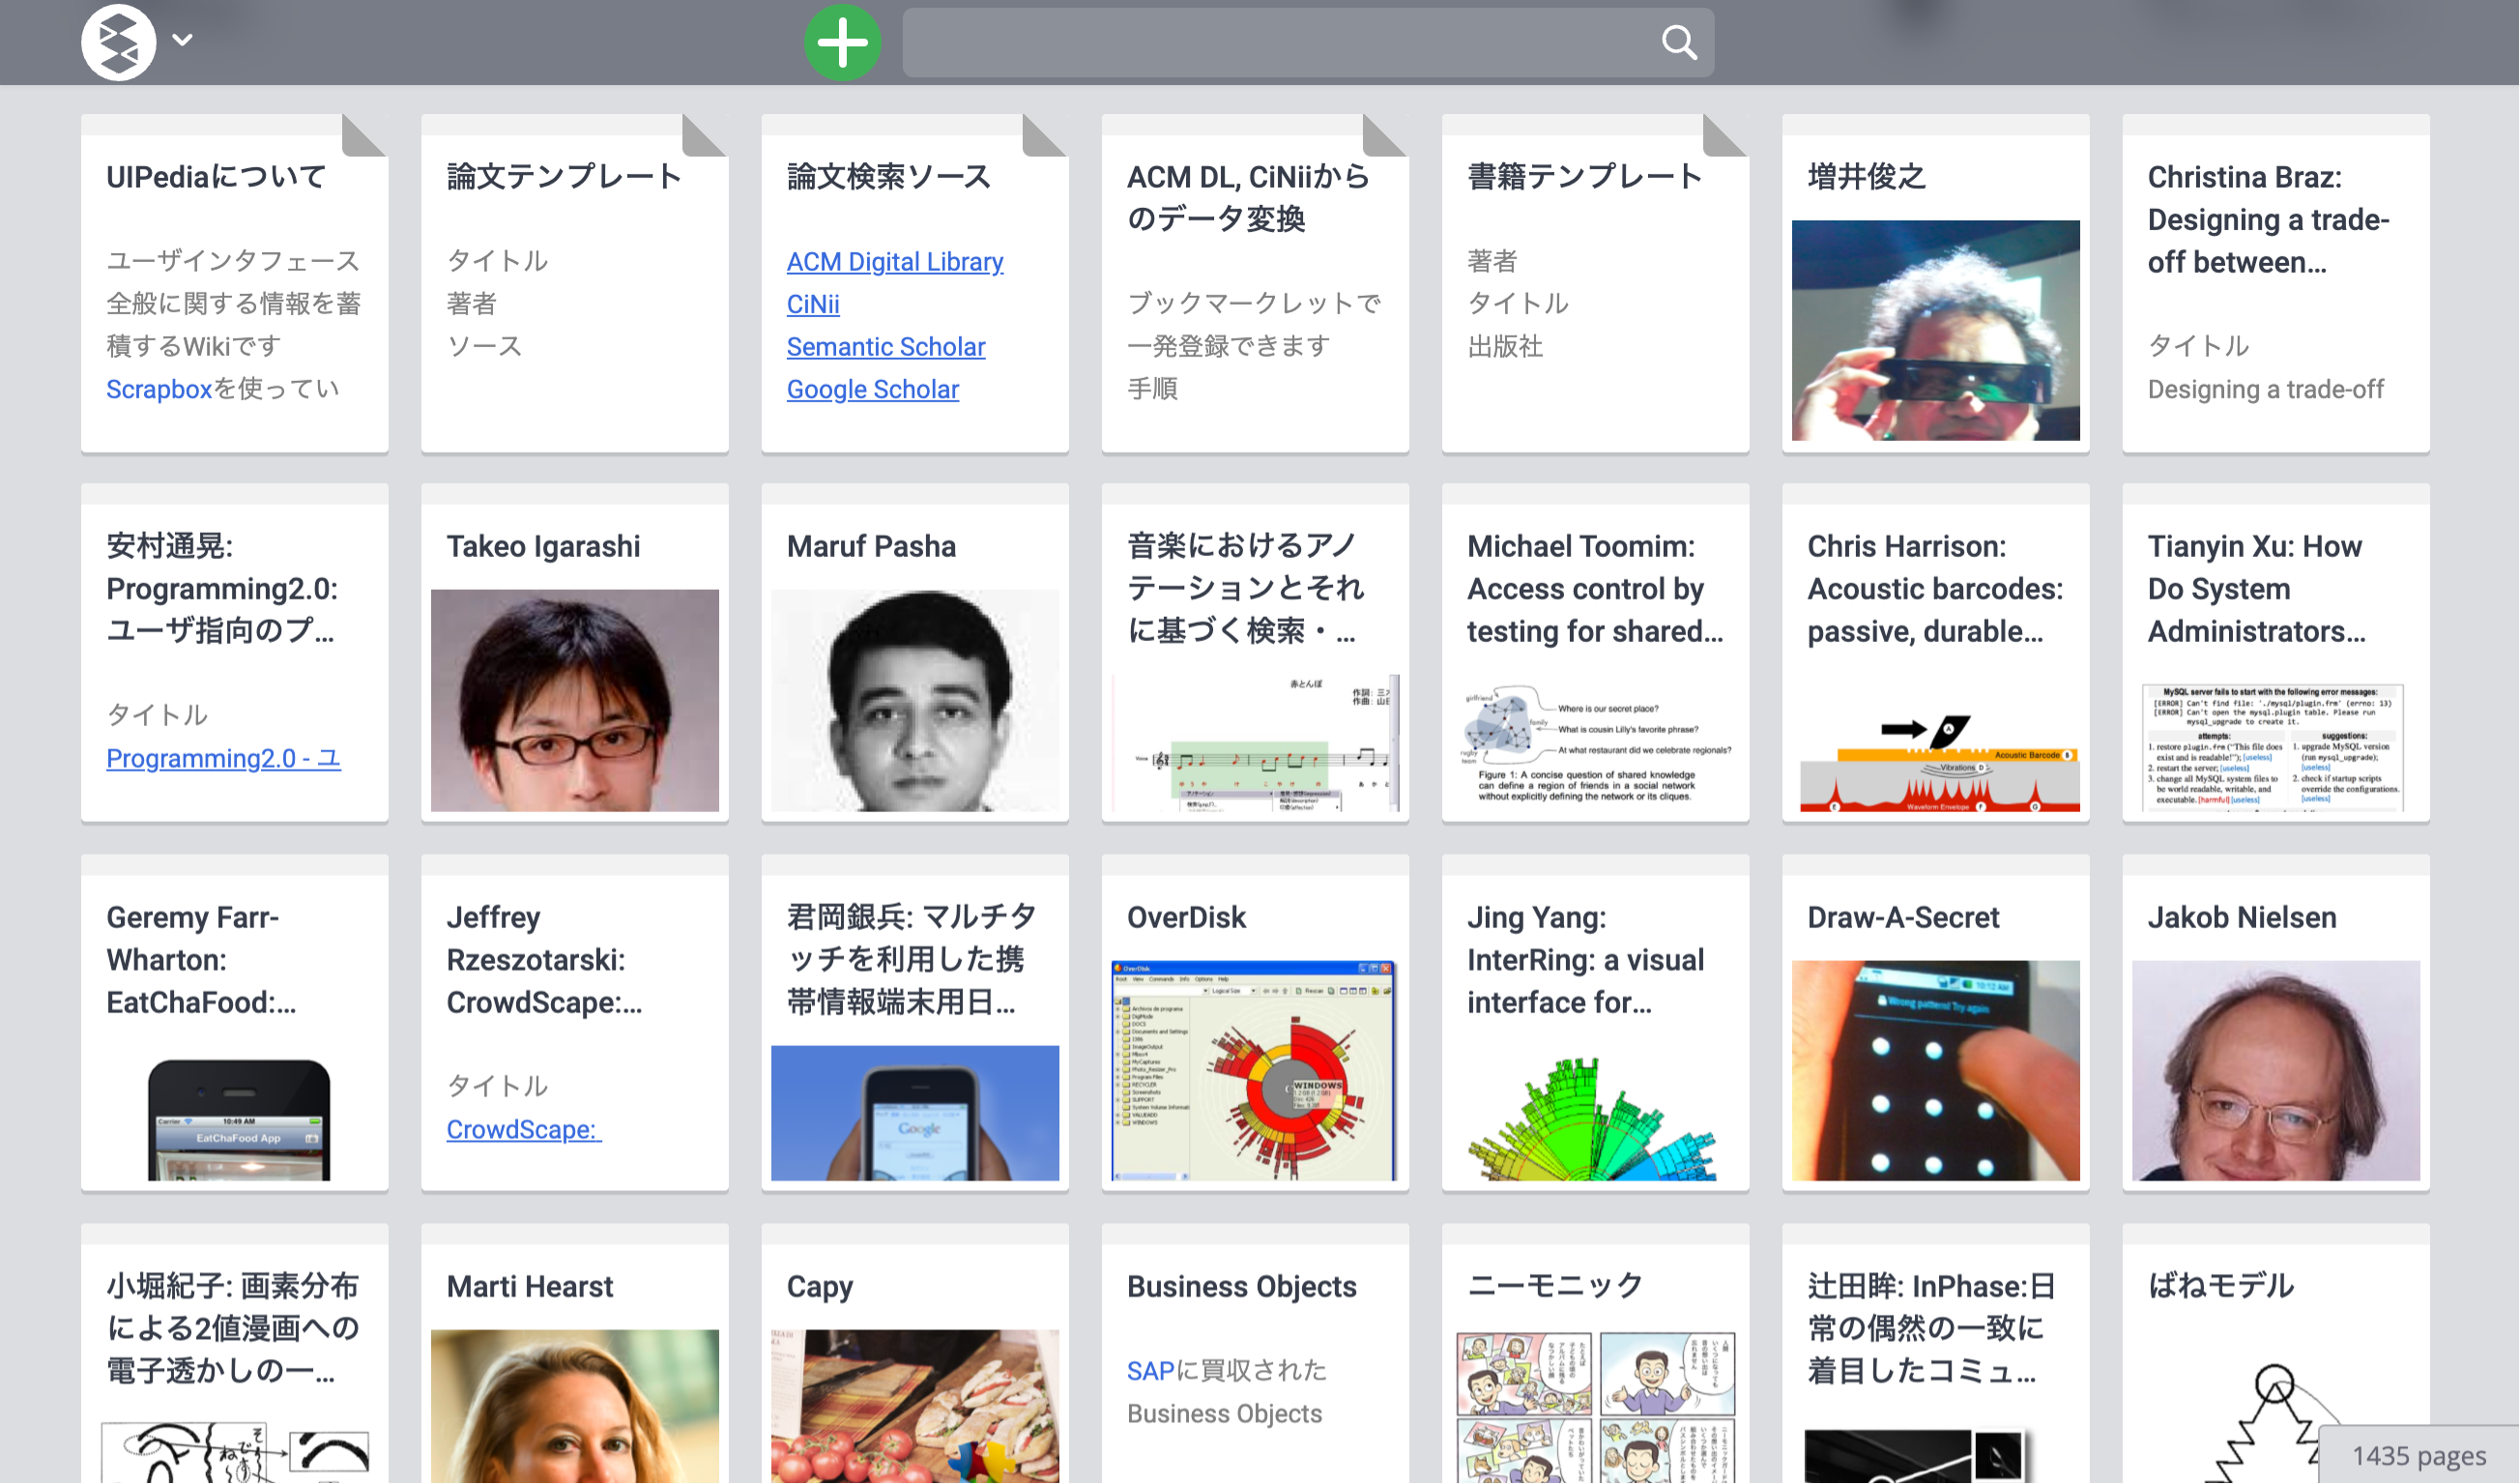
\includegraphics[width=9cm,bb=0 0 2607 1535]{figures/13982c755fdc0c60af2548c0a6589543.png}
  \caption{Scrapboxを使った情報整理の例}
  \label{example1}
\end{figure}

\begin{figure}[t]
  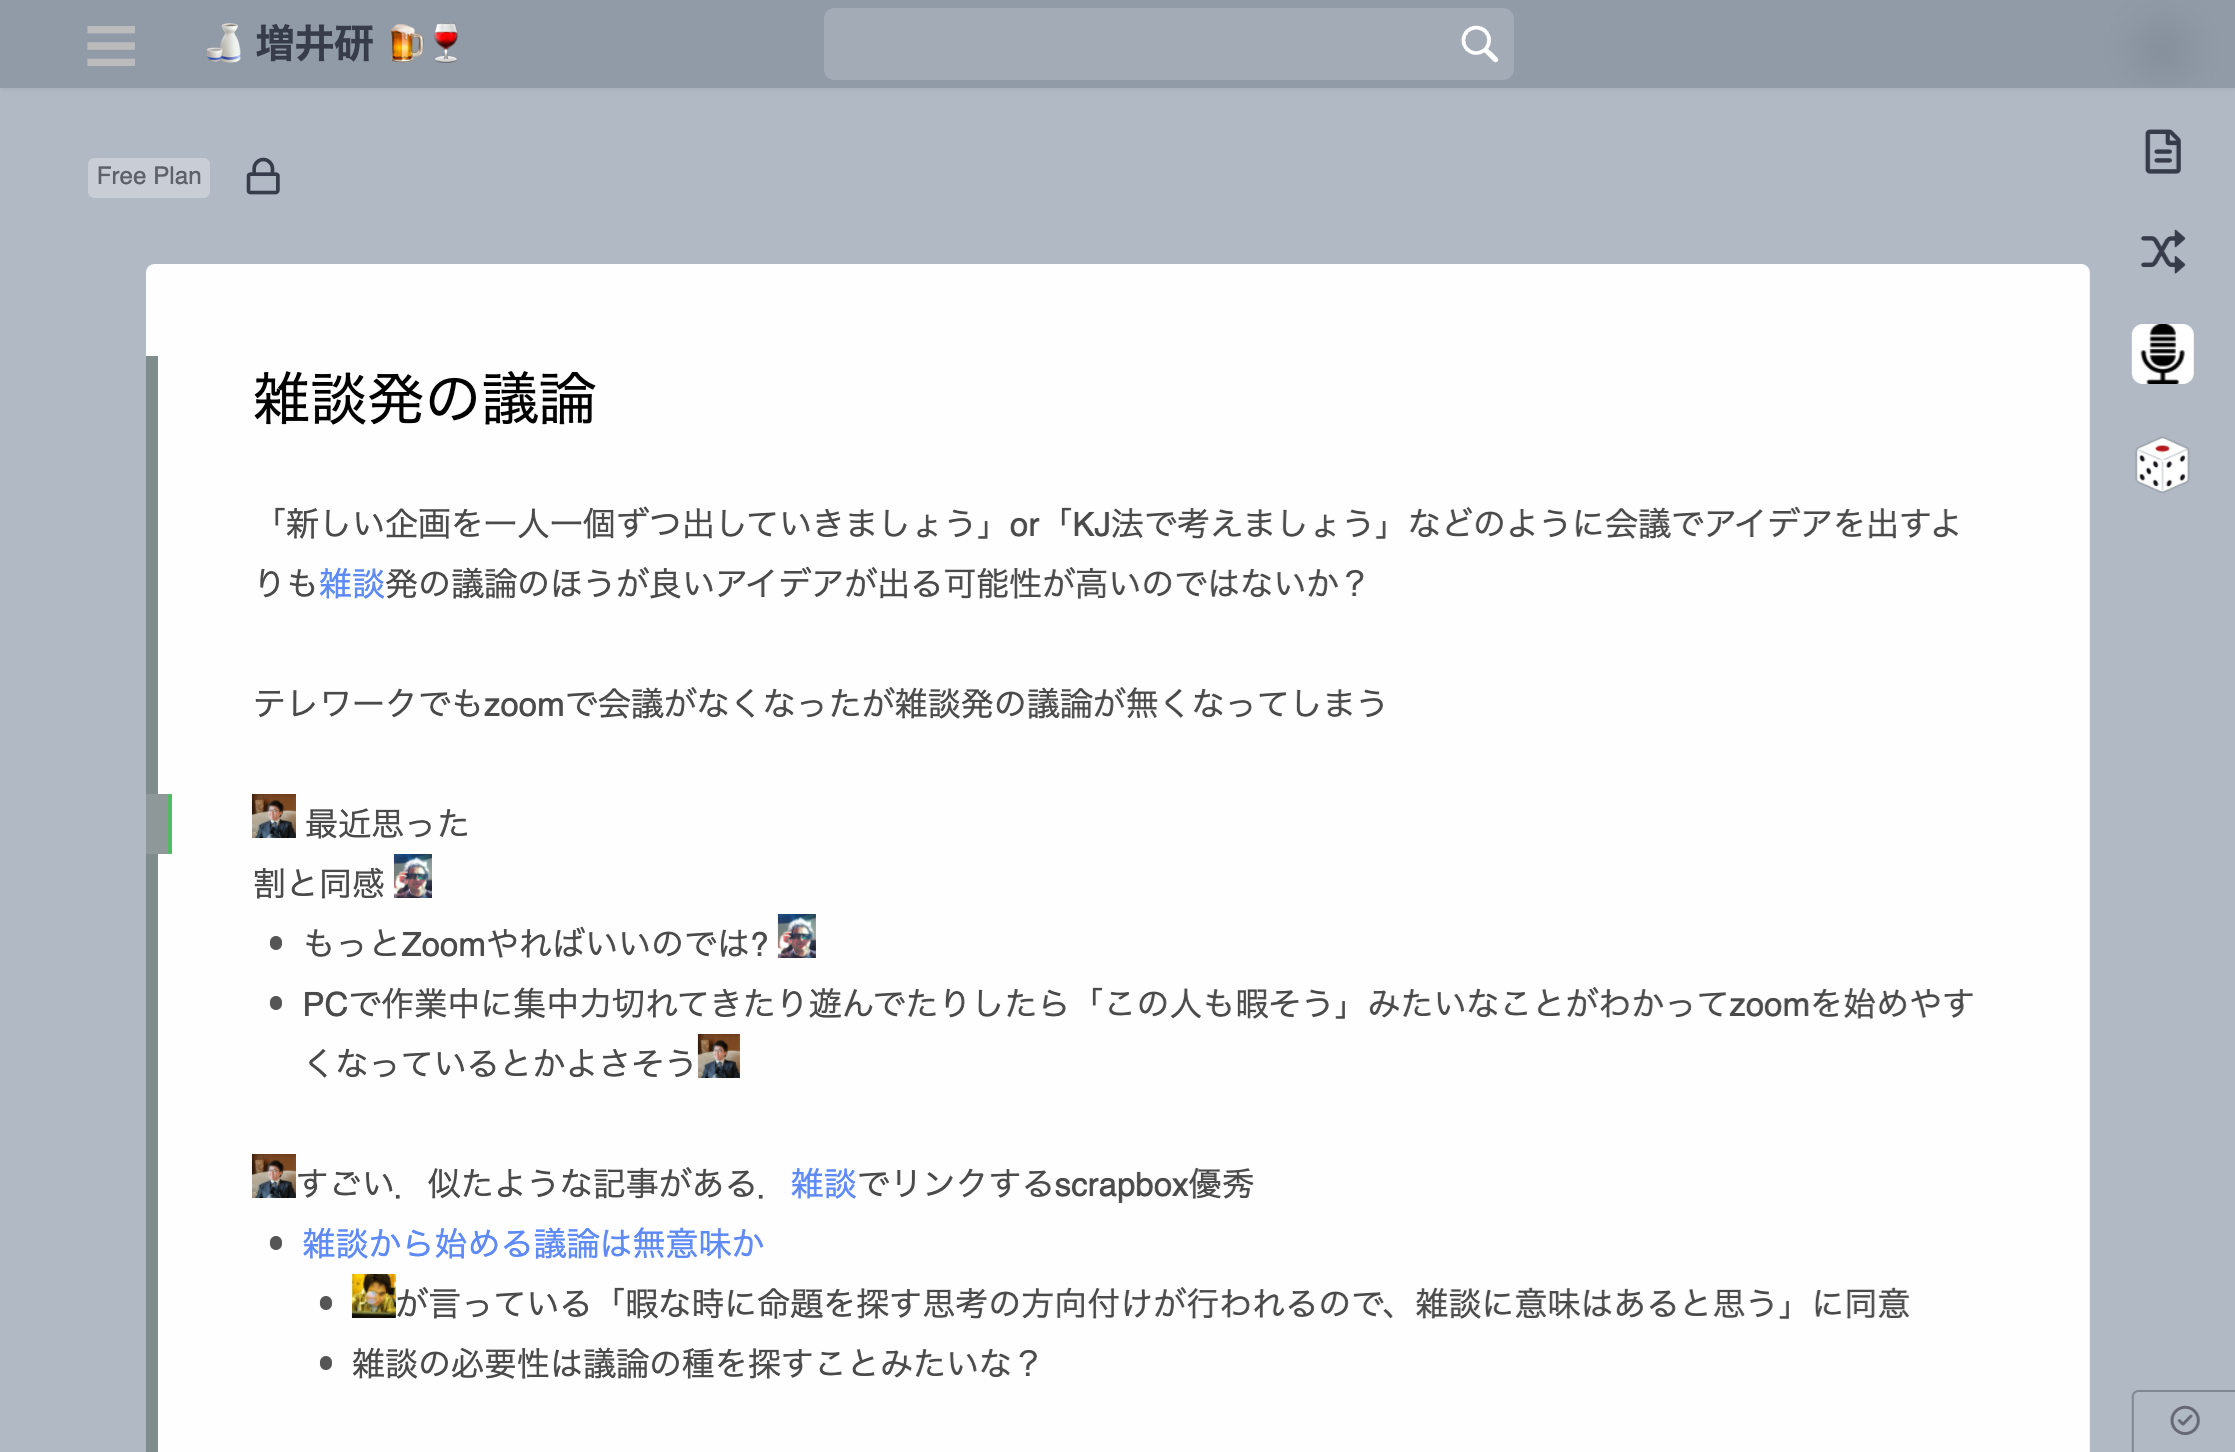
\includegraphics[width=9cm,bb=0 0 2235 1452]{figures/cca2e0eaed298ea4952a26d2effa238c.png}
  \caption{Scrapboxを使った情報整理}
  \label{example1}
\end{figure}

リアルタイムにWikiを利用できると情報整理にとても便利です。
様々なデータをカードに記述し、
それらを利用してアイデアをまとめる作業は
梅棹忠夫氏の「知的生産の技術」\footnote{
  \textsf{https:{\slash}{\slash}www.amazon.co.jp{\slash}dp{\slash}4004150930}
}や「Zettelkasten」\footnote{
  \textsf{https:{\slash}{\slash}en.wikipedia.org{\slash}wiki{\slash}Zettelkasten}
}で提案され、広く利用されてきました。
これらは紙ベースのものですが、ScrapboxはこれをWikiで実現することにより、
柔軟で有用なシステムとなっています。

\subsection{検索支援}

複雑なシステムやサービスが身のまわりに増えてきていますが、
使い方などがわからないとき問題を解決する方法はまだまだ不充分です。
大抵のパソコンOSやアプリケーションにはヘルプ機能が用意されていますが、
ヘルプシステムを使って問題が解決できることは少ないので、
ほとんど使われていないようで、
GoogleなどでWeb検索したり他人に聞いたりすることで問題を解決してることがほとんどです。

\begin{figure}[t]
  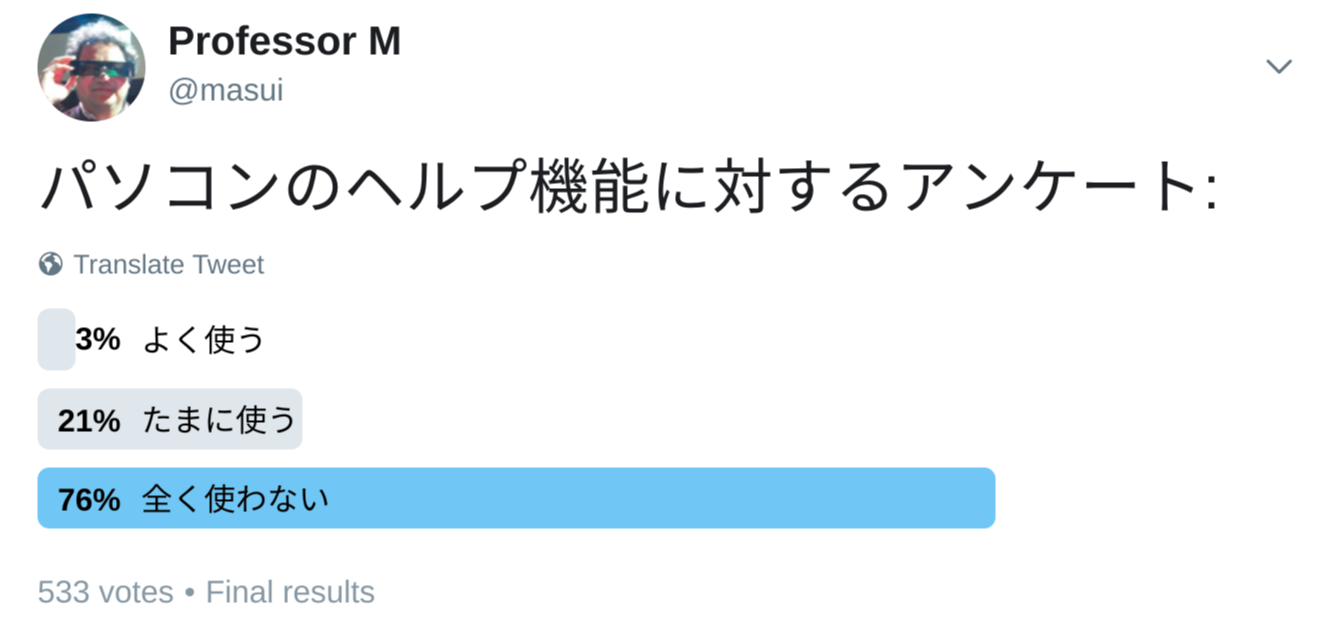
\includegraphics[width=9cm,bb=0 0 1332 623]{figures/383ee54c265ebbb88778d7ea0fbea5b1.png}
  \caption{ヘルプ機能の利用状況アンケート (2019/2/28)}
  \label{helpinquiry}
\end{figure}

ヘルプの検索にはキーワード検索を使うことが多いですが、
ユーザの頭の中の単語とヘルプ文書中の単語は一致しないのが普通なので、
必要な情報をうまくみつけるのは困難です\cite{10.1145/32206.32212}。

このような問題を解決するため、
頭の中に出現しそうなキーワードにマッチするあらゆるヘルプ文書を用意しておき、
キーワードと曖昧検索を行なうことによりヘルプを実現する
「展開ヘルプ」\cite{ExpandHelp}技術を開発し、
「Helpfeel」という商品名でサービスをしています。

\subsection{コンテンツ閲覧}

最近のネットには大量のコンテンツが存在し、
パソコンやテレビでそれらを楽しむことができますが、
コンテンツを選択するための操作は難しいのが普通です。

ふたつのキーだけを利用して大量のコンテンツを選択して楽しむことができる
「Serencast」システムを開発しました\cite{Serencast}。
Serencastを利用すると、
複雑なリモコン操作を全くせずに大量のコンテンツをブラウジングできます。

\begin{figure}[t]
  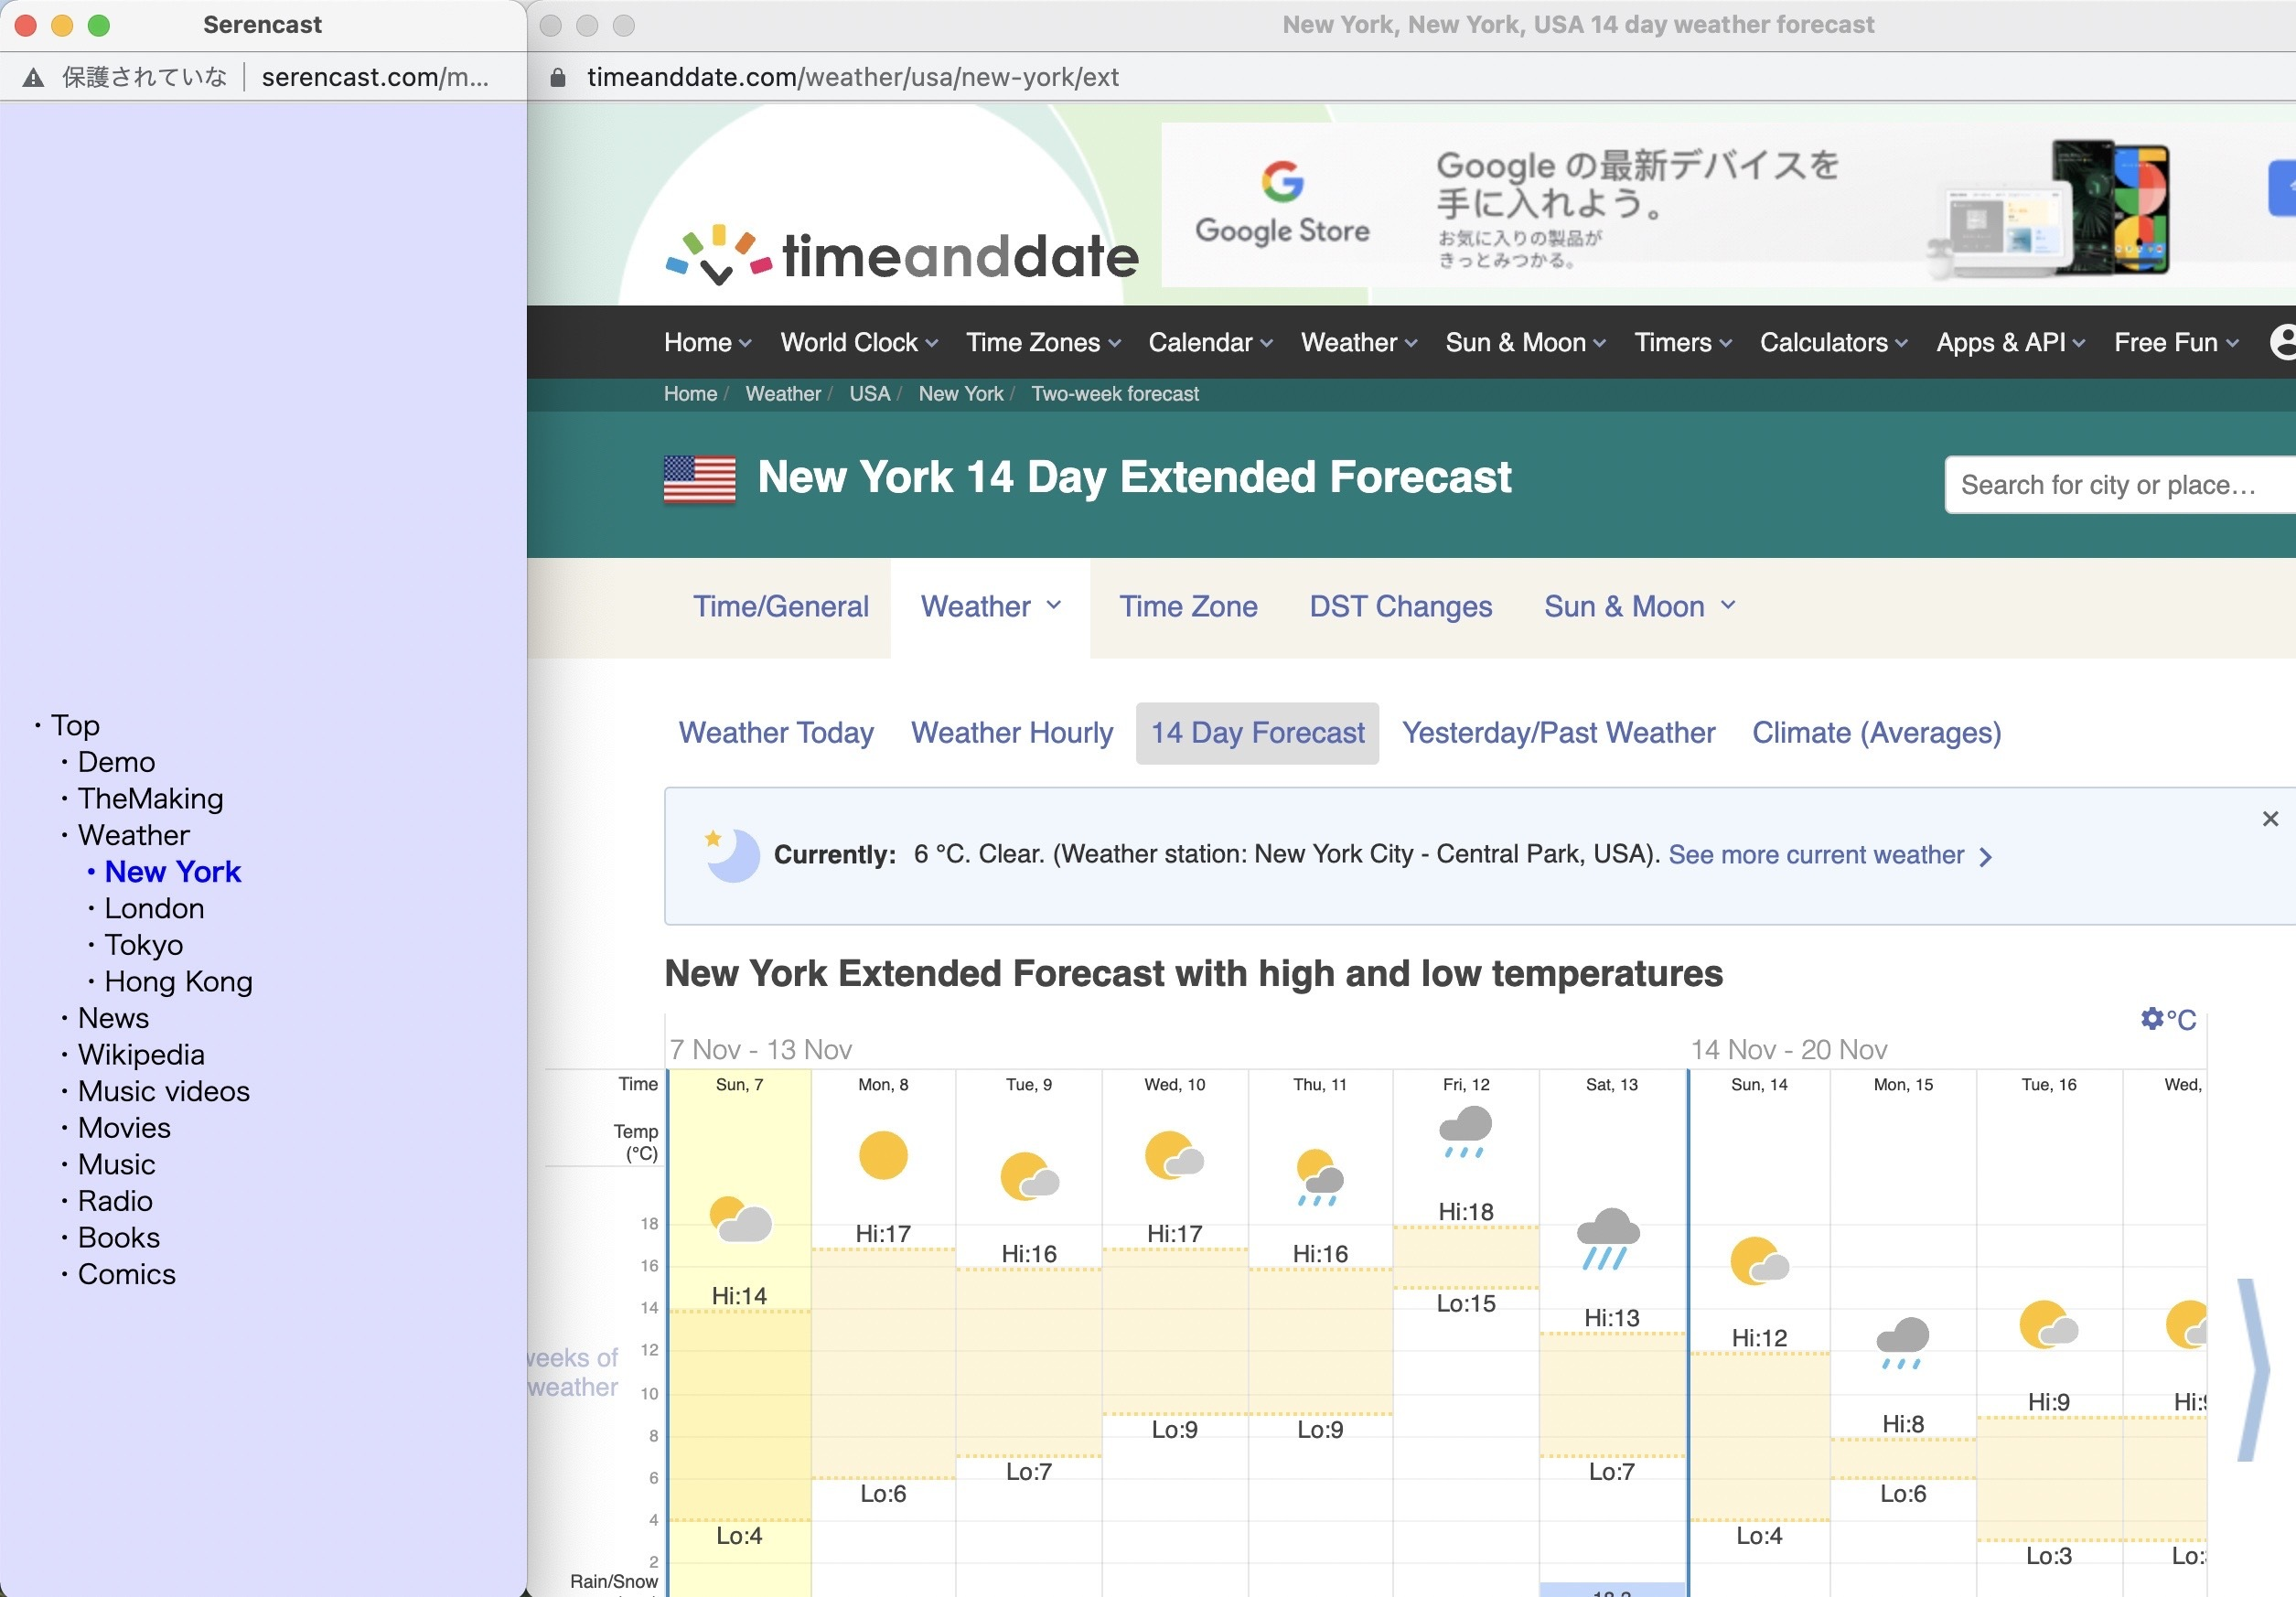
\includegraphics[width=9cm,bb=0 0 2510 1746]{figures/bb4027e2e210bc16450f0120a2987458.jpg}
  \caption{Serencast}
  \label{example1}
\end{figure}

\subsection{パスワード管理}

ネット上のサービスを利用するとき
サービスごとに異なるIDやパスワードが必要になることが多く、
パスワードの管理が大変になってきています。
従来はパスワードは人間の頭で覚えることになっていましたが、
サービスの種類だけパスワードを覚えることは不可能になっています。
異なるサービスで同じパスワードを利用することは危険なので、...

沢山のパスワードを利用するためには
「パスワード管理システム」が広く利用されています。
しかし、パスワード管理システムを利用するためにパスワードが必要ですし、
特殊なアプリケーションはどこでも使えるとは限りません。

こういう問題を解決するために、
既に自分が覚えているエピソード記憶からパスワードを生成して利用できる
「EpisoPass」というシステムを開発しました。
自分だけが覚えているエピソード記憶を利用して...

\section{まとめ}

長年にわたり、誰もがいつでもどこでも利用できる
ユニバーサルなアプリケーションやサービスの開発に勤めてきました。
有用なアプリケーションを作成するためには
基礎的なコンピュータサイエンスの技術が必要です。

\bibliographystyle{jssst}
\bibliography{paper}

\par

\chosha{増井俊之}{
  1984年東京大学大学院工学系研究科電子工学専門課程修士課程修了。 工学博士。
  シャープ、ソニーコンピュータサイエンス研究所、産業技術総合研究所、Apple Inc.などに勤務後、
  2009年4月より慶應義塾大学]環境情報学部教授。
  情報検索、テキスト入力、情報視覚化、実世界指向インタフェース、予測インタフェース、認証技術など、
  ユーザインタフェースに関連する幅広い研究開発を行なっている。
  携帯電話やスマートフォンで広く利用されている予測入力システムPOBoxや
  フリック入力システムの開発者。
  Gyazo, Scrapbox, Helpfeel, EpisoPass, 本棚.orgなど
  各種のWebサービスを運用中。
  WISSの話も書く
  }
  
\end{document}

% https://scrapbox.io/masui/%E3%82%BD%E3%83%95%E3%83%88%E3%82%A6%E3%82%A7%E3%82%A2%E7%A7%91%E5%AD%A6%E4%BC%9A_%E5%9F%BA%E7%A4%8E%E7%A0%94%E7%A9%B6%E8%B3%9E%E8%AC%9B%E6%BC%94
